\section*{\nr.3 \titthree (10 Punkte)}
\begin{enumerate}[(a)]
\item
Das durch den ersten Polarisator dringende Licht habe die Intensität $I_1$. Nach dem Gesetz von Malus gilt für die resultierende Intensität nach einem zweiten Polarisator, der relativ zum ersten um den Winkel $\theta$ verdreht ist:
\begin{equation}
I' = I \cos^2{\theta}
\end{equation}
Zweimaliges Anwenden liefert als resultierende Intensität $I_\text{res}$ für die Anordnung in \vref{fig:polar3}:
\begin{equation}
I_\text{res} = I_1 \cos^2{(\pi/4)} \cdot \cos^2{(\pi/4)} = \frac{1}{4}I_1
\end{equation}
\begin{figure}[htbp]
\centering
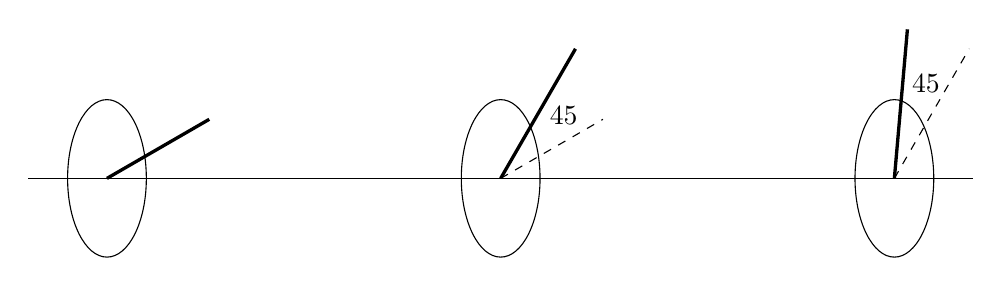
\begin{tikzpicture}
%Hauptachse und Polarisatoren
\draw (0,0) -- (12,0);
\draw (1,0) circle[x radius = 5mm, y radius = 10mm];
\draw (6,0) circle[x radius = 5mm, y radius = 10mm];
\draw (11,0) circle[x radius = 5mm, y radius = 10mm];
%Winkelandeutungen
\draw[very thick] (1,0) -- ++(30:1.5cm);
\draw[dashed] (6,0) -- ++(30:1.5cm);
\draw[very thick] (6,0) -- ++(60:1.9cm);
\node at (6.8,0.8) {$\ang{45}$};
\draw[dashed] (11,0) -- ++(60:1.9cm);
\draw[very thick] (11,0) -- ++(85:1.9cm);
\node at (11.4,1.2) {$\ang{45}$};
\end{tikzpicture}
\caption{Hintereinanderschaltung von drei Polarisatoren. Die fette Linie beim jeweiligen Polarisator deutet die Transmissionsachse an.}
\label{fig:polar3}
\end{figure}
\item
Für die Anordnung in \vref{fig:polar4} berechnet sich die resultierende Intensität als:
\begin{equation}
I_\text{res} = I_1 \left(\cos^2{(\pi/6)}\right)^3 = \frac{27}{64} I_1
\end{equation}
\begin{figure}[htbp]
\centering
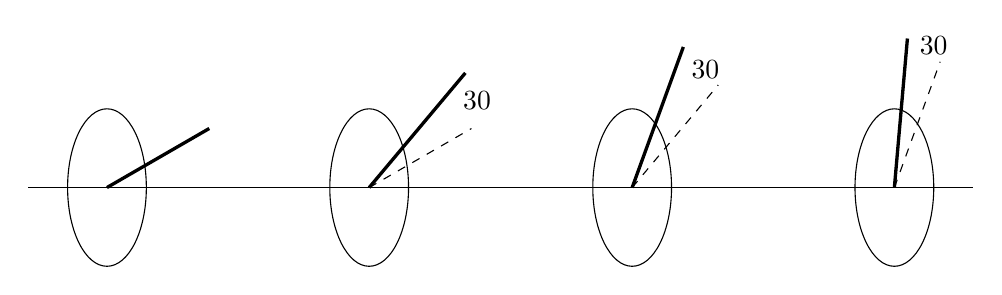
\begin{tikzpicture}
%Hauptachse und Polarisatoren
\draw (0,0) -- (12,0);
\draw (1,0) circle[x radius = 5mm, y radius = 10mm];
\draw (4.33,0) circle[x radius = 5mm, y radius = 10mm];
\draw (7.67,0) circle[x radius = 5mm, y radius = 10mm];
\draw (11,0) circle[x radius = 5mm, y radius = 10mm];
%Winkelandeutungen
\draw[very thick] (1,0) -- ++(30:1.5cm);

\draw[dashed] (4.33,0) -- ++(30:1.5cm);
\draw[very thick] (4.33,0) -- ++(50:1.9cm);
\node at (5.7,1.1) {$\ang{30}$};

\draw[dashed] (7.67,0) -- ++(50:1.7cm);
\draw[very thick] (7.67,0) -- ++(70:1.9cm);
\node at (8.6,1.5) {$\ang{30}$};

\draw[dashed] (11,0) -- ++(70:1.7cm);
\draw[very thick] (11,0) -- ++(85:1.9cm);
\node at (11.5,1.8) {$\ang{30}$};
\end{tikzpicture}
\caption{Hintereinanderschaltung von vier Polarisatoren. Die fette Linie beim jeweiligen Polarisator deutet die Transmissionsachse an.}
\label{fig:polar4}
\end{figure}
\item Zuletzt werden $n-1$ Polarisatoren eingebracht, die je um den Winkel $\pi/(2n)$ verdreht sind. Als resultierende Intensität des passierenden Lichts ergibt sich:
\begin{equation}
I_\text{res} = I_1 \left(\cos^2{\left(\frac{\pi}{2n}\right)}\right)^n = I_1 \left( \cos\frac{\pi}{2n} \right)^{2n}
\end{equation}
Zur Betrachtung des Grenzprozesses $n\to \infty$ entwickeln wir den Kosinusterm an der Stelle Null:
\begin{align}
\left(\cos{\frac{\pi}{2n}}\right)^{2n} &\approx \left(1-\frac{\pi^2}{2\cdot (2n)^2}\right)^{2n} = \left(1-\frac{\pi^2}{2\cdot (N)^2}\right)^{N} \\
\intertext{mit $N:=2n$. Der binomische Lehrsatz liefert:}
\left(1-\frac{\pi^2}{2\cdot (N)^2}\right)^{N} &= 1- \frac{\pi^2 N}{2 N^2} +\frac{\pi^4 N(N-1)}{8 N^4} \mp \dots \\
&= 1+ \mathcal{O}\left(\frac{1}{N}\right)
\end{align}
Also gilt für den zu untersuchenden Grenzprozess:
\begin{equation}
\lim_{n\to\infty} I_1 \left( \cos\frac{\pi}{2n} \right)^{2n} = \lim_{N\to\infty} I_1\left[1+ \mathcal{O}\left(\frac{1}{N}\right) \right] =I_1
\end{equation}
Bemerkenswerterweise kann also bei unendlich vielen Polarisatoren alles Licht passieren.
\end{enumerate}